%%%%%%%%%%%%%%%%%%%%%%%%%%%%%%
% CORESIDENCE RATES FOR M/F  %
%%%%%%%%%%%%%%%%%%%%%%%%%%%%%%
\begin{figure}[H]
  \caption{Coresidence Rates by Age and Gender} 
  \label{fig:cores_rates}
  \begin{center}
    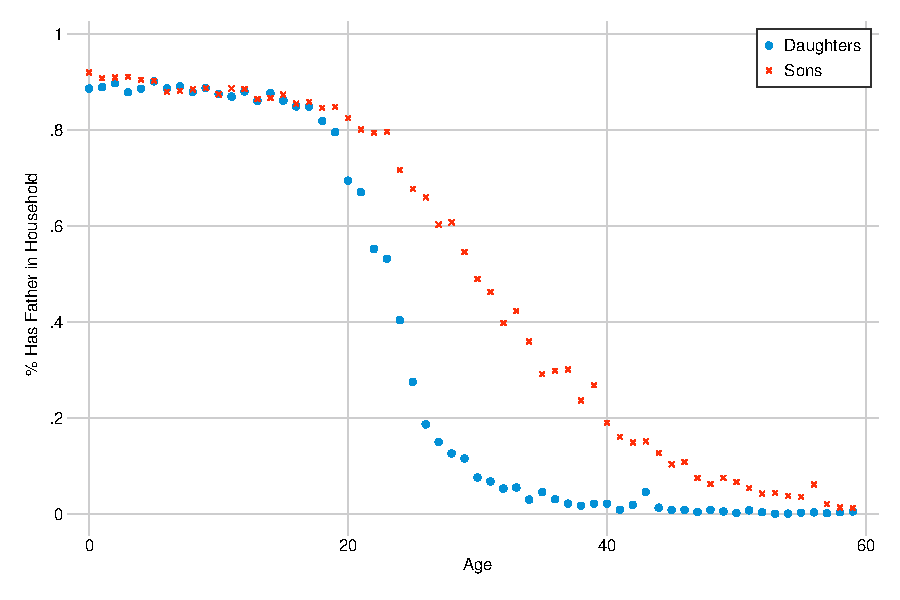
\includegraphics[scale=0.5]{\mobilitypath/cores_age}
  \end{center}
  \newline
  \footnotesize{Figure~\ref{fig:cores_rates} shows the share of
    individuals who live in the same household as their father as a
    function of gender and age. Source: IHDS (2012).}  
\end{figure}

%%%%%%%%%%%%%%%%%%%%%%%%%%%%%%%%%%%%%%
% CORESIDENCE BIAS IN MOB ESTIMATES  %
%%%%%%%%%%%%%%%%%%%%%%%%%%%%%%%%%%%%%%
\begin{figure}[h]
  \caption{Bias in Mobility Estimates When Sample is Limited to Coresident Pairs} 
  \label{fig:cores_bias}

  \begin{center}
    \begin{tabular}{cc}
      A. Father-Son Pairs &        B. Father-Daughter Pairs  \\
      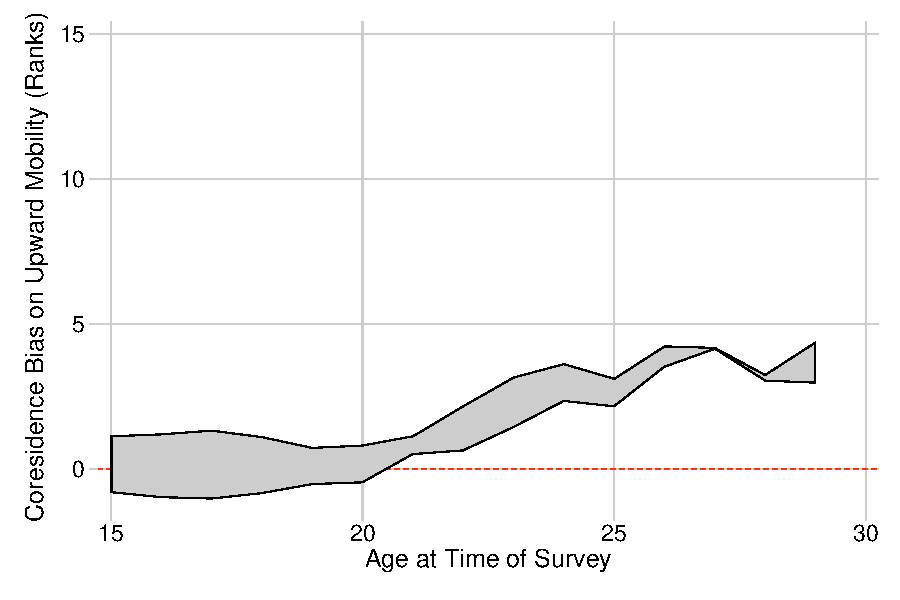
\includegraphics[scale=0.45]{\mobilitypath/cores_bias_upward_m} & 
      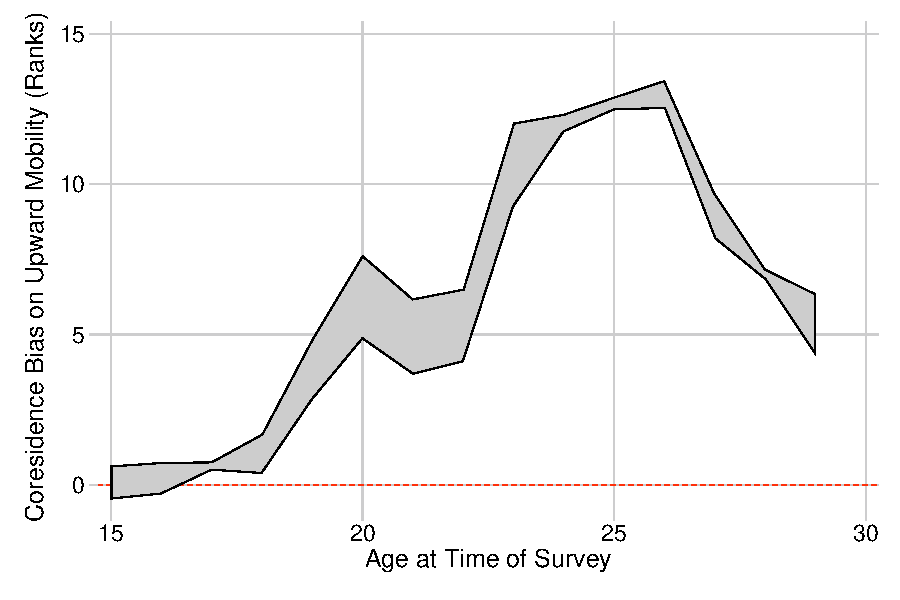
\includegraphics[scale=0.45]{\mobilitypath/cores_bias_upward_f} \\
      \end{tabular}          
  \end{center}
  \newline
  \footnotesize{Figure~\ref{fig:cores_bias} shows the bias in a
    measure of upward mobility when children who do not live with
    their parents are excluded from the sample. The bias is shown as a function of
    child age. The mobility measure is bottom half mobility
    ($\mu_0^{50}$), which is the expected child rank conditional on
    being born to a parent in the bottom half of the education
    distribution. Bias is calculated as the coresident-only measure
    minus the full sample measure. Source: IHDS (2012).}
\end{figure}

%%%%%%%%%%%%%%%%%%%%%%%%%%%%%%
%% RANK-RANK SCATTER GRAPHS %%
%%%%%%%%%%%%%%%%%%%%%%%%%%%%%%
\begin{landscape}
  \begin{figure}[h]
    \vspace{-2cm}
  \caption{Joint Parent-Child Education Moments Over Time} 
  \label{fig:rank_scatters}

  \begin{center}
    \begin{tabular}{cc}
      \panel{A. Father-Son Pairs} &       \panel{B. Father-Daughter Pairs} \\ 
      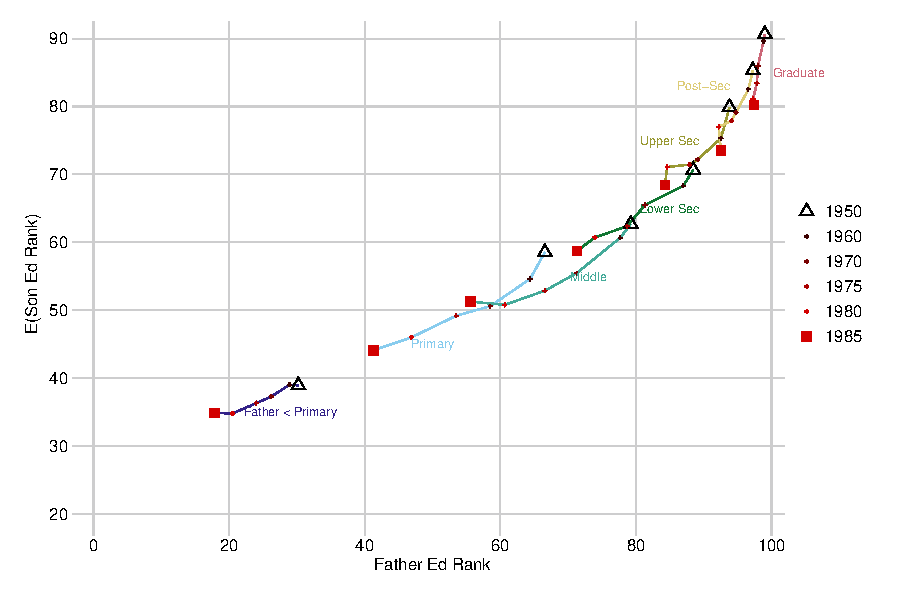
\includegraphics[scale=0.7]{\mobilitypath/scatter_father_son} & 
      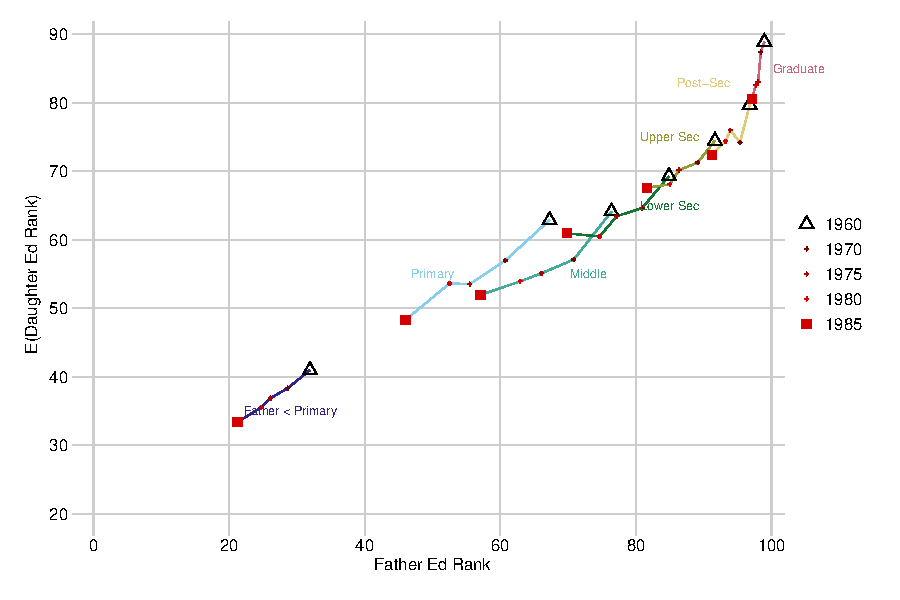
\includegraphics[scale=0.7]{\mobilitypath/scatter_father_daughter} \\
      \panel{C. Mother-Son Pairs} &       \panel{D. Mother-Daughter Pairs} \\ 
      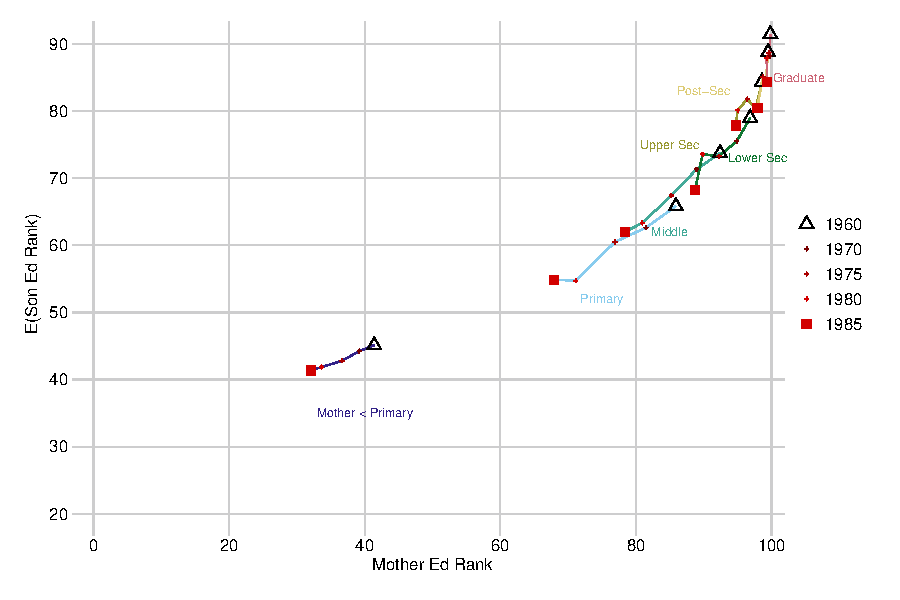
\includegraphics[scale=0.7]{\mobilitypath/scatter_mother_son} & 
      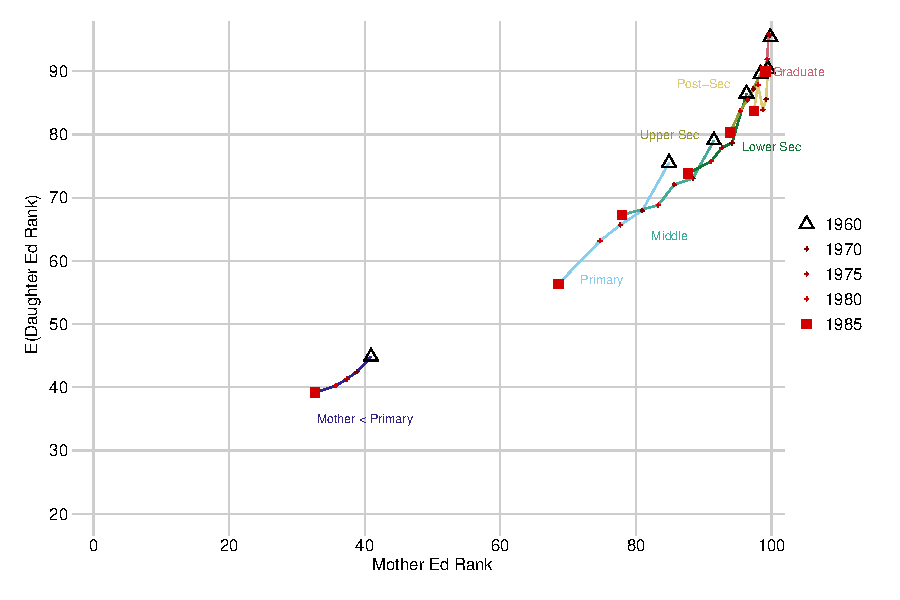
\includegraphics[scale=0.7]{\mobilitypath/scatter_mother_daughter} \\
    \end{tabular}
  \end{center}
  \newline
  \footnotesize{The figure shows the conditional expectation function of child education rank, given parent education rank for six cohorts. Each set of connected points corresponds to a time series for a different \textit{level} of education; the time series (which moves from the triangle to the square) shows changes in a child's expected rank (Y axis) given a parent at some fixed level of education, along with the change in the father's education rank (X axis) in the cohort of fathers. Points move to the southwest because low-education fathers have lower ranks as education rises (moving left), and thus have children with lower education ranks (moving down). Ranks are calculated as the midpoint rank of a given education bin. Source: IHDS (2012).}
\end{figure}
\end{landscape}
\resetgeometry
%%%%%%%%%%%%%%%%%%%%%%%%%%%%%%%%%%%%%%%%%%%
%% SURVIVOR BIAS: IHDS 2005 vs IHDS 2011 %%
%%%%%%%%%%%%%%%%%%%%%%%%%%%%%%%%%%%%%%%%%%%
\newpage 
\begin{figure}[H]
  \caption{Robustness of Upward Mobility to Survivorship Bias} 
  \label{fig:mob_survivor}

  \begin{center}
    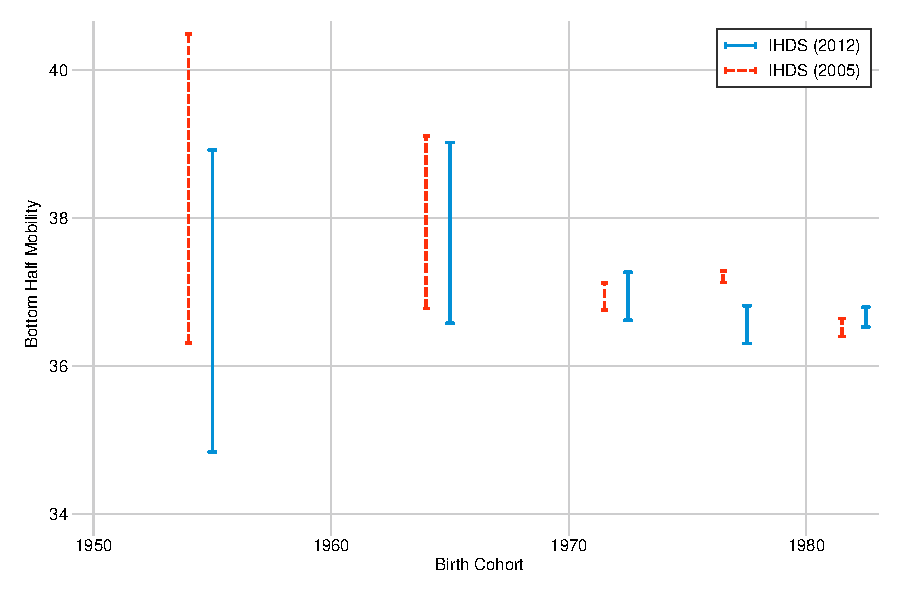
\includegraphics[scale=0.5]{\mobilitypath/mob_survivor} \\
  \end{center}
  \footnotesize{Figure \ref{fig:mob_survivor} shows a test of
    survivorship bias in estimates of bottom half mobility. The figure
    shows estimates of bottom half mobility calculated for the 1950s to 1980--85
    birth cohorts, measured separately in the 2005 and 2012 rounds of the IHDS. If there
    was substantial survivorship bias in the mobility measures, we
    would expect the estimates to differ across the two surveys
    because of the deaths of some of the respondents.}
\end{figure}

%%%%%%%%%%%%%%%%%%%%%
%% MOTHERS MU-0-50 %%
%%%%%%%%%%%%%%%%%%%%%
\begin{figure}[h]
  \caption{Bottom Half Mobility ($\mu_0^{50}$) for Mother-Son and
    Mother-Daughter Pairs } 
  \label{fig:mob_moms_mu50}

  \begin{center}
    \begin{tabular}{cc}
      A. Mother-Son Pairs &       B. Mother-Daughter Pairs \\ 
      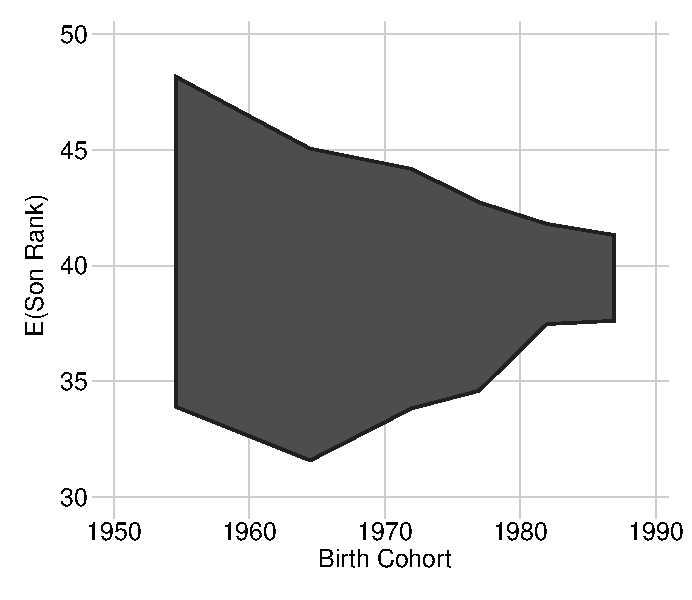
\includegraphics[scale=0.5]{\mobilitypath/ihds_mob_time_ms} & 
      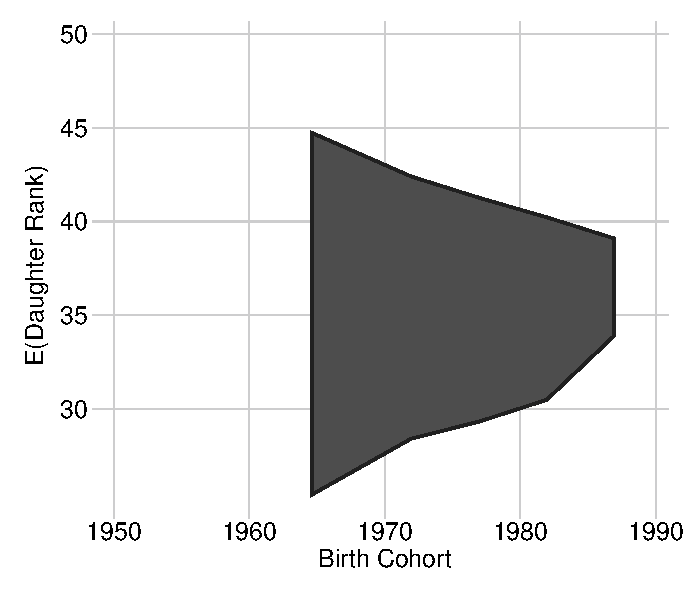
\includegraphics[scale=0.5]{\mobilitypath/ihds_mob_time_md} \\
      \end{tabular}          
  \end{center}
  \newline
  \footnotesize{Figure \ref{fig:mob_moms_mu50} shows bounds on
    aggregate trends in intergenerational mobility, using cohorts born
    from 1950--59 through 1985--89, focusing on mother-son and
    mother-daughter links. The measure used is bottom half mobility
    ($\mu_{0}^{50}$), which is the average rank attained by children
    born to parents who are in the bottom half of the education
    distribution. The bounds are very wide because of the large share
    of mothers who report bottom-coded education levels. Source: IHDS (2012).}
\end{figure}

%%%%%%%%%%%%%%%%%%%%%%%%%%%%%%%%%%%%%%%%%%%%%%
%% TRENDS BY SOCIAL GROUP -- LEVEL OUTCOMES %%
%%%%%%%%%%%%%%%%%%%%%%%%%%%%%%%%%%%%%%%%%%%%%%
\clearpage
\newpage 
\begin{figure}[H]
  \caption{Trends in Mobility by Subgroup, 1950--1989 Birth Cohorts
    \cnewline Education Level Outcomes} 
  \label{fig:group_mob_levels}

  \begin{center}
    \begin{tabular}{cc}
      
      \panel{A. Father-Son, Primary School $\boldsymbol \mu_0^{50}$} &
      \panel{B. Father-Daughter, Primary School $\boldsymbol \mu_0^{50}$}    \\ 
      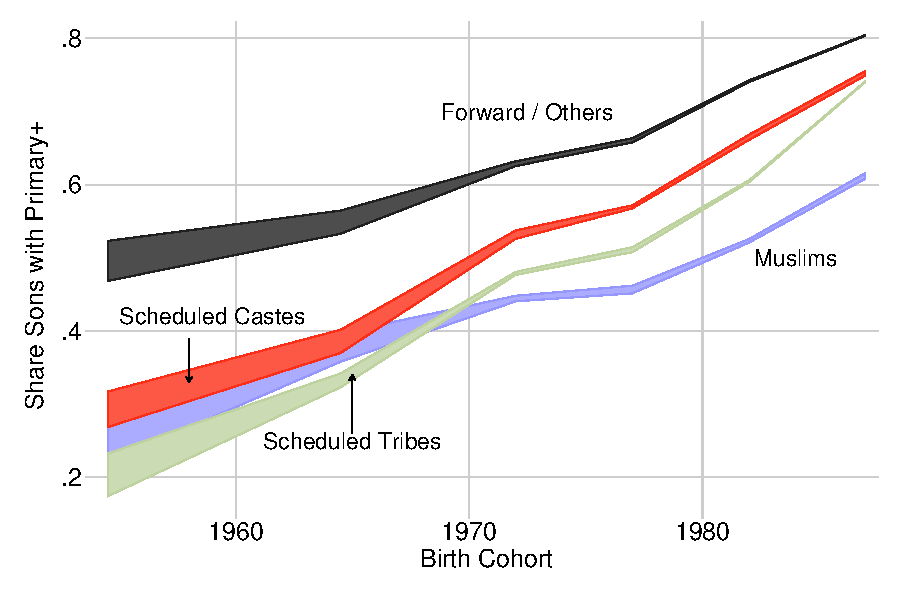
\includegraphics[scale=0.55]{\mobilitypath/ihds_mob_group_time_p25_prim_m} &
      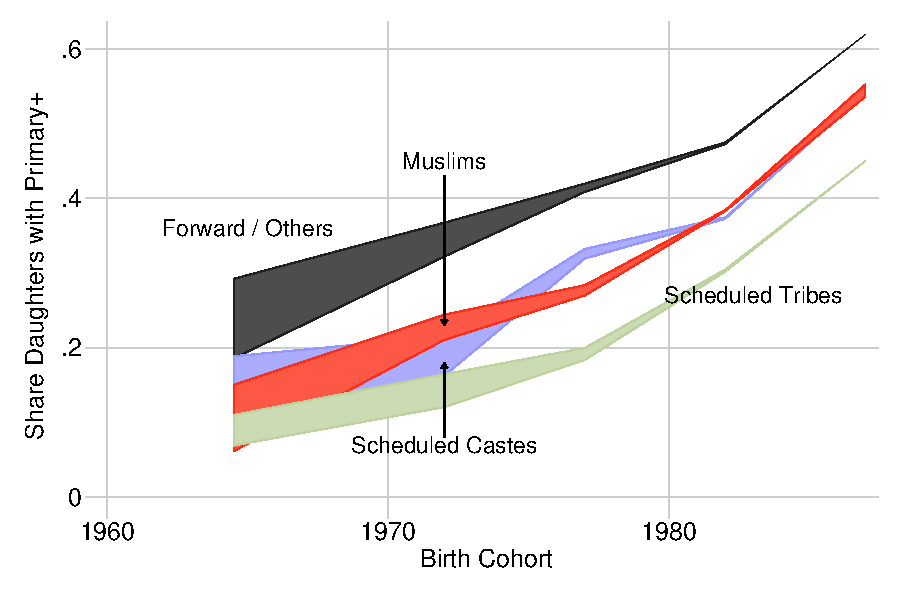
\includegraphics[scale=0.55]{\mobilitypath/ihds_mob_group_time_p25_prim_f}
      \\
      
      \panel{C. Father-Son, High School $\boldsymbol \mu_0^{50}$} &
      \panel{D. Father-Daughter, High School $\boldsymbol \mu_0^{50}$}    \\ 
      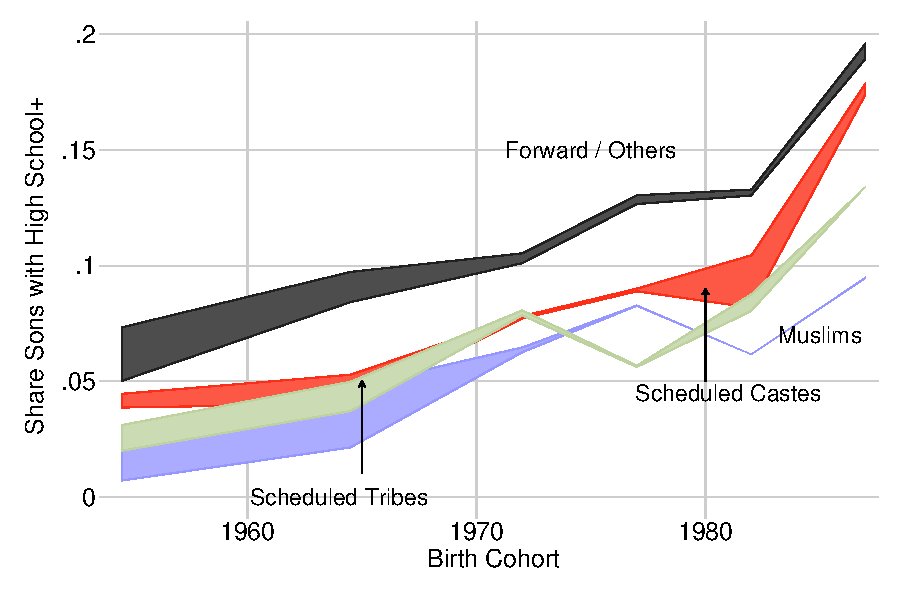
\includegraphics[scale=0.55]{\mobilitypath/ihds_mob_group_time_p25_hs_m} &
      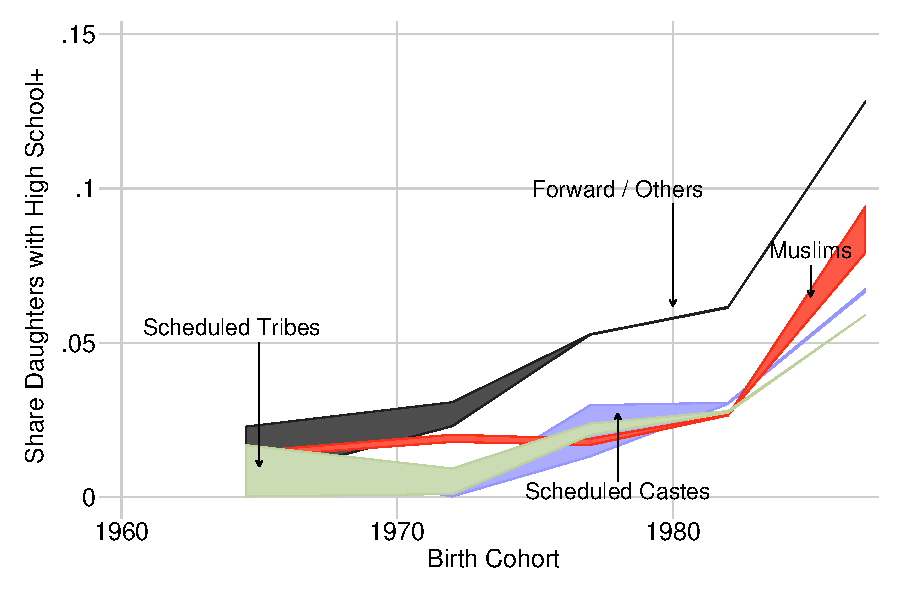
\includegraphics[scale=0.55]{\mobilitypath/ihds_mob_group_time_p25_hs_f}
      \end{tabular}          
  \end{center}
  \newline
  \footnotesize{Figure \ref{fig:group_mob_levels} presents bounds on 
    intergenerational mobility, stratified by four prominent social
    groups in India: Scheduled Castes, Scheduled Tribes, Muslims, and
    Forward Castes/Others. The figure is analogous to
    Figure~\ref{fig:group_mob}, but shows the expected probability that a child
    attains a given education level (primary
    in Panels A and B, and secondary in Panels C
    and D), conditional on having a 
    father in the bottom half of the father education
    distribution. Linked father-daughter education data are not
    available for the 1950--59 birth cohort.
    Source: IHDS (2012).}
\end{figure}

%%%%%%%%%%%%%%%%%%%%%%%%%%%%%%%%%%%%%%%%%%%%%%%%%%%%%%%%%%%%%%%%
%% Cassan affirmative action spec with a range of post values %%
%%%%%%%%%%%%%%%%%%%%%%%%%%%%%%%%%%%%%%%%%%%%%%%%%%%%%%%%%%%%%%%%
\newpage 
\begin{figure}[H]
  \caption{Effect of Scheduled Caste Designation on Upward Mobility \cnewline
  Robustness to Alternate Post Years} 
  \label{fig:aa_by_post}

  \begin{center}
    \begin{tabular}{c}
      \panel{A. Father-son pairs} \\
      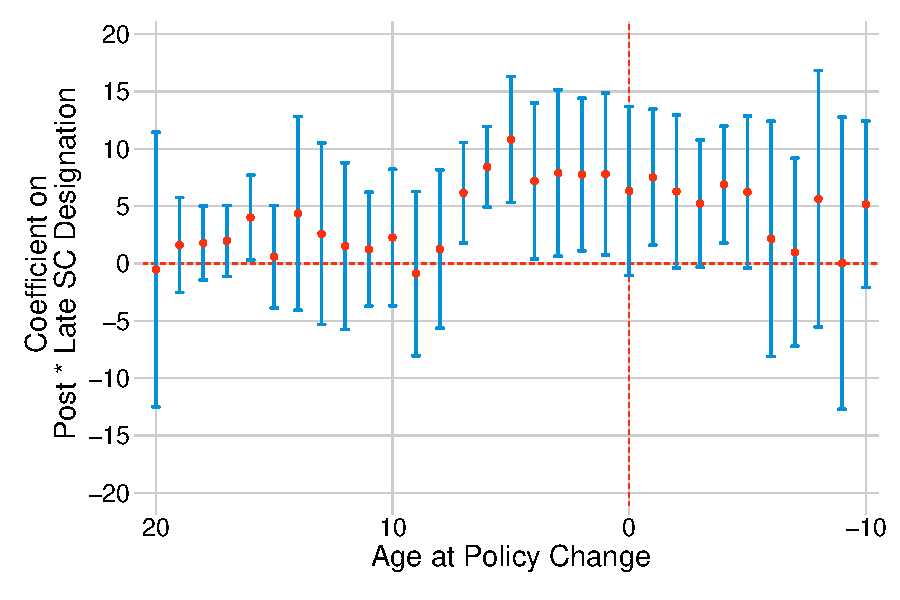
\includegraphics[scale=0.55]{\mobilitypath/aa_time_series_boy} \\
      \panel{B. Father-daughter pairs} \\
      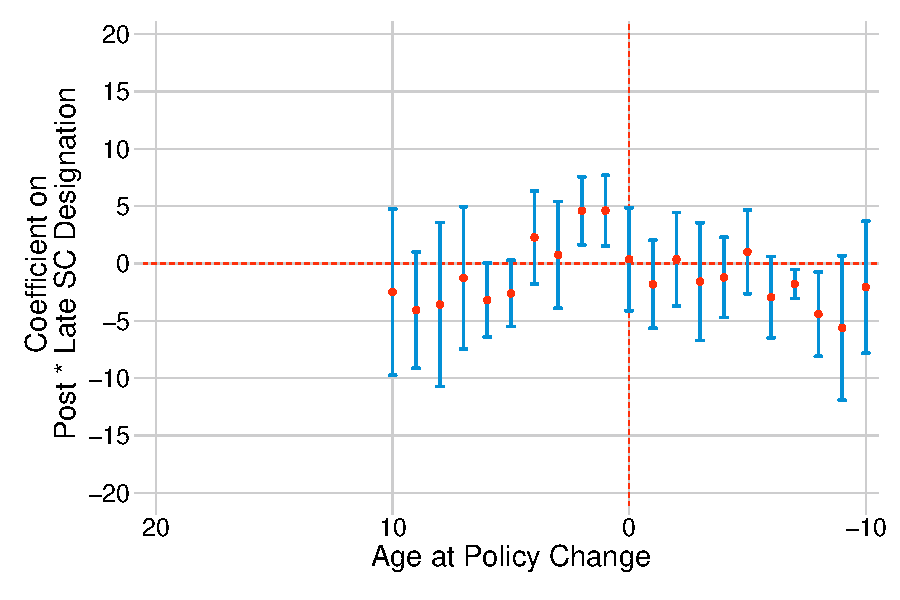
\includegraphics[scale=0.55]{\mobilitypath/aa_time_series_girl}
      \end{tabular}          
  \end{center}
  \newline
  \footnotesize{The figure shows point estimates from Equation~\ref{eq:cassan}, with a range of definitions of ``post'', the first year at which post-policy-change cohorts are modeled as exposed to the new policy regime. The X axis shows the child's age at the time of the policy change in 1977; negative ages describe children born after 1977. All outcomes are measured in 2012. The Y axis shows a regression coefficient which describes the relative gains in rank points to ``Late'' Scheduled Caste children born after their castes were added to the Scheduled Caste list (see Section~\ref{sec:cassan}). Source: IHDS (2012).}
\end{figure}

%%%%%%%%%%%%%%%%%%%%%%%%%%%%%%%%%%%%%%%%%%%%%%%%%%%
%% Rejected mechanisms for mobility differences  %%
%%%%%%%%%%%%%%%%%%%%%%%%%%%%%%%%%%%%%%%%%%%%%%%%%%%
\begin{landscape} 
\begin{figure}
\caption{Other Candidate Mechanisms}
  \label{fig:mechanisms}
  \begin{center}
    \begin{tabular}{cc}
      \panel{A. Within-State and Within-District Social Group Mobility Gaps}  &
      \panel{B. Mincerian Returns for Different Social Groups}  \\
      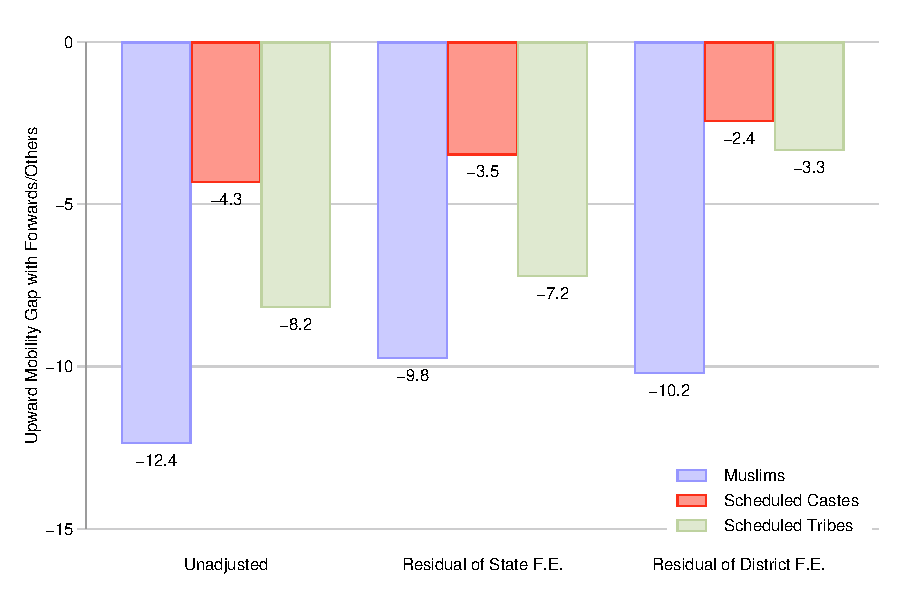
\includegraphics[scale=0.65]{\mobilitypath/mob_gaps_sd_resids} &
      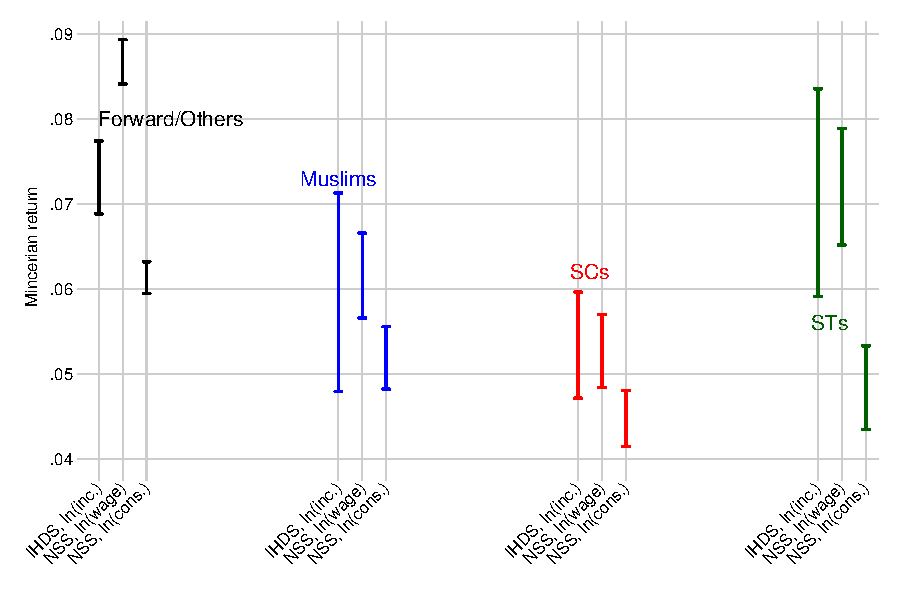
\includegraphics[scale=0.65]{\mobilitypath/mincerian_returns_pooled_4} \\
      \panel{C. Business Ownership by Demographic Group} &
      \panel{D. Mobility by Business Ownership} \\
      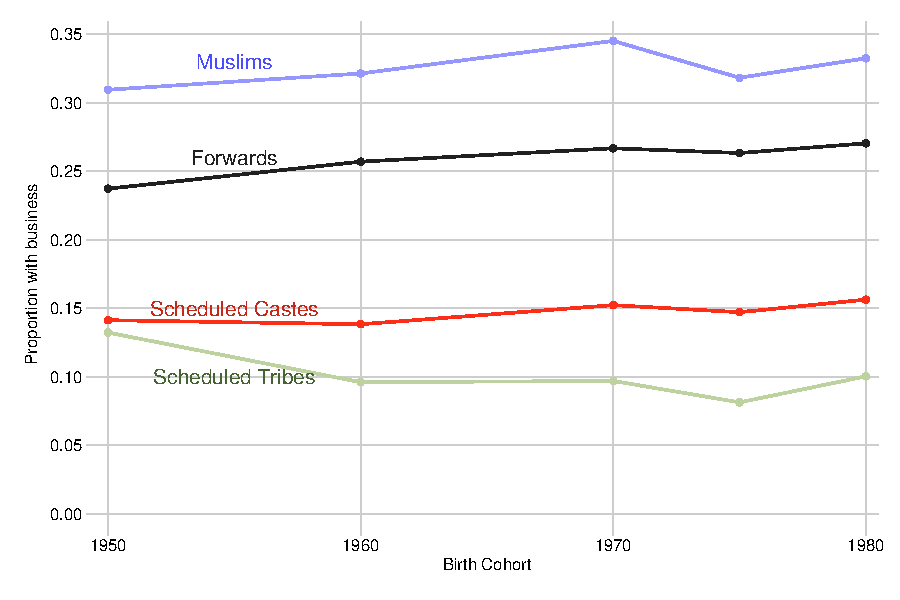
\includegraphics[scale=0.65]{\mobilitypath/has_business_ts} & 
      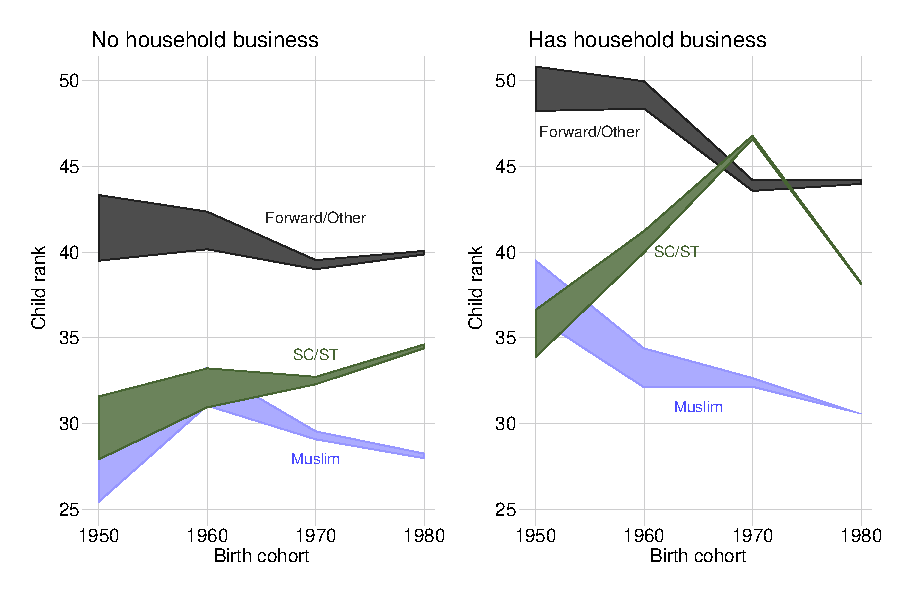
\includegraphics[scale=0.65]{\mobilitypath/mob_by_own_business} \\
  \end{tabular}
\end{center}
  \newline
  \tiny{Panel A presents the bottom-half mobility disadvantage relative to Forwards/Others faced by Muslims, Scheduled Castes and Scheduled Tribes. The first set of bars shows the average national mobility ranks. Upward mobility for the Forward/Others reference group is 42. Upward mobility is partially identified; we show the midpoint of the bounds, which in all cases span less than a single rank point. The following two sets of bars are calculated using within-state and within-district education ranks; they describe mobility gaps that are entirely within states and districts respectively.  Panel B shows 95\%
    confidence intervals for the Mincerian return to household log income
    (IHDS 2012), individual log wages (NSS 2012), and household log
    per capita income (NSS 2012). Panel C shows the share
    of individuals who report that they work in their own business, by
    social group and time. Panel D shows bottom
    half mobility for the major social groups,
    separated by individual business ownership. Scheduled Castes and
    Tribes are pooled to increase power, since few members of either
    group own businesses. Source for Panels C and D: NSS 2012.}
\end{figure}
\end{landscape} 


